\documentclass[11pt,a4paper]{article}

\usepackage[margin=2.4cm]{geometry}
\usepackage{graphicx}
\usepackage{booktabs}
\usepackage{amsmath}
\usepackage[T1]{fontenc}
\usepackage{microtype}
\usepackage{xcolor}
\usepackage[colorlinks=true,allcolors=blue!55!black]{hyperref}
\usepackage{caption}
\captionsetup{font=small,labelfont=bf}

\setlength{\parskip}{0.45em}
\setlength{\parindent}{0pt}

\title{\vspace{-1.4cm}\textbf{windcheck}\\[0.25em]
\large Label-free detection of cross-wrap self-coincidence\\
in Herculaneum scroll segmentations}
\author{Josep Carreras}
\date{July 2026}

\begin{document}
\maketitle
\vspace{-0.9em}

\section*{Summary}

A traced papyrus surface that goes once around the scroll should come back onto
the \emph{next} sheet. \texttt{windcheck} finds the places where it comes back
onto the \emph{same} sheet instead.

The check runs on the published \texttt{tifxyz} meshes alone. It needs no
ground-truth labels, no annotations, no trained model, no GPU, and no volume
download: a full scroll of 53 surfaces is analysed in a few minutes on a laptop
from about 670\,MB of surface data. It ships with a calibration command, a null
control that passes, and a validity filter that refuses to report rows it cannot
stand behind.

This addresses Open Problems \S2 and \S3 --- \emph{``sheet switches, where a
traced mesh jumps from the intended sheet to a neighboring wrap''} and mesh
topology repair, described there as \emph{``one of the highest-leverage places
to contribute.''}

\section{The problem}

A scroll is one sheet, rolled. Segmentation traces that sheet through the CT
volume. When a tracer crosses to an adjacent wrap, the output still looks like a
clean surface, and the text rendered from it still looks like text --- but it is
spliced from two different parts of the scroll. The failure is silent, which is
what makes it expensive.

There is no published set of known-bad segments, so a supervised detector cannot
be trained and a supervised evaluation cannot be run. Any usable check must
therefore be derived from a property the correct answer must satisfy, and must
carry its own controls.

\section{Method}

A \texttt{tifxyz} surface is a 2D grid of 3D vertex coordinates: grid index
$(v,u)$ maps to a volume coordinate. Walking along $u$ goes around the scroll.

For every grid point $p$, measure the distance to the nearest point of
\emph{the same surface} that is at least $E$ grid columns away in $u$:
\[
g(p) \;=\; \min_{\;|u_q - u_p| \ge E} \; \lVert p - q \rVert ,
\qquad q \in S .
\]
The exclusion removes the patch of surface $p$ already sits on, so what remains
is the trace's own neighbouring wrap. A correct trace reads one sheet spacing
there. A value near zero means the trace is lying on top of a wrap it has
already traced.

Two properties of this definition matter.

\textbf{It never needs a scroll axis.} An earlier version of this work measured
radius against winding number instead. That approach fails its own positive
control: fitting radius on the 44 labelled sheets of Scroll~5 --- ground truth,
known radial order --- leaves a residual standard deviation of 79.8 voxels
against a sheet spacing of 12--17 voxels, because a carbonised scroll is
crushed, not round. Comparing a trace to itself is invariant to that
deformation.

\textbf{Distance is measured to the interpolated surface}, not to the nearest
grid sample. The grids are sampled roughly every 20 voxels while adjacent sheets
sit about 17 voxels apart, so a nearest-sample method has less than a $1.5\times$
margin and cannot separate one sheet of gap from two.

The kernel is C++17 with a uniform-grid acceleration structure and a
\texttt{std::thread} pool, sustaining roughly 27{,}000 point-to-surface queries
per second on 12 threads against a 30-million-triangle atlas.

\section{Calibration}

Thresholds are meaningless until the scroll says what a sheet is worth. The
\texttt{calibrate} command measures the distance from each labelled winding to
the sheet $k$ windings away.

\begin{table}[h]
\centering
\small
\begin{tabular}{lrrr}
\toprule
separation & surface pairs & median distance & ratio \\
\midrule
1 sheet  & 43 & 17.05\,vx & 1.000 \\
2 sheets & 42 & 34.14\,vx & 2.003 \\
3 sheets & 41 & 51.22\,vx & 3.004 \\
\bottomrule
\end{tabular}
\caption{Sheet separation on \texttt{PHerc0172}, over 126 surface pairs. The
linearity is what licenses reading a doubled gap as a skipped wrap. If it does
not hold on a given scroll, the labels are not a radial index and the check does
not apply there.}
\end{table}

\begin{figure}[h]
\centering
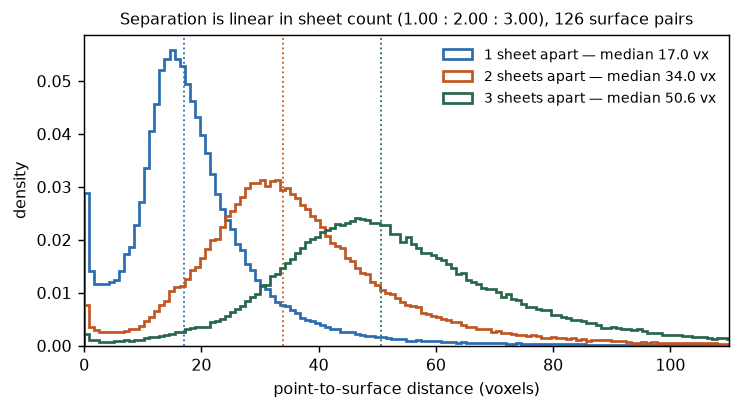
\includegraphics[width=0.82\textwidth]{img/calibration.png}
\caption{The same measurement as distributions. The overlap is shown
deliberately: per-\emph{point} discrimination between a one- and two-sheet gap
is only about 78\%, which is why every verdict in this work is made over a
region and never over a single point.}
\end{figure}

\section{Controls}

\textbf{Null control.} A single-wrap segment has no previous wrap, so a working
check must find nothing on it. All 44 labelled single-winding segments of
Scroll~5 report 0.00\% flagged. The same property is pinned by a unit test on a
synthetic flat sheet, so it cannot silently regress.

\textbf{Validity filter.} Exclusion by $u$-index assumes $u$ advances with
angle. Where that assumption is weak, a flagged partner may be a same-wrap
neighbour rather than the next wrap. Any trace whose flagged $|\Delta u|$ tenth
percentile falls within $2E$ is rejected --- in code, not by inspection.

The filter is not decorative. On \texttt{PHerc0814} it rejects the two
\emph{highest-scoring} traces (11.27\% and 8.18\% of points inside the
2.0-voxel threshold), both artifacts of the exclusion cutoff. Without it, they
would have been the headline numbers of this submission.

\textbf{Cross-check.} On the traces that pass, flagged partners sit at
$|\Delta u| = 271$--$618$ columns, matching revolution periods derived
independently by angular unwrapping ($236$--$616$) across all nine traces.

\section{Results}

\begin{figure}[h]
\centering
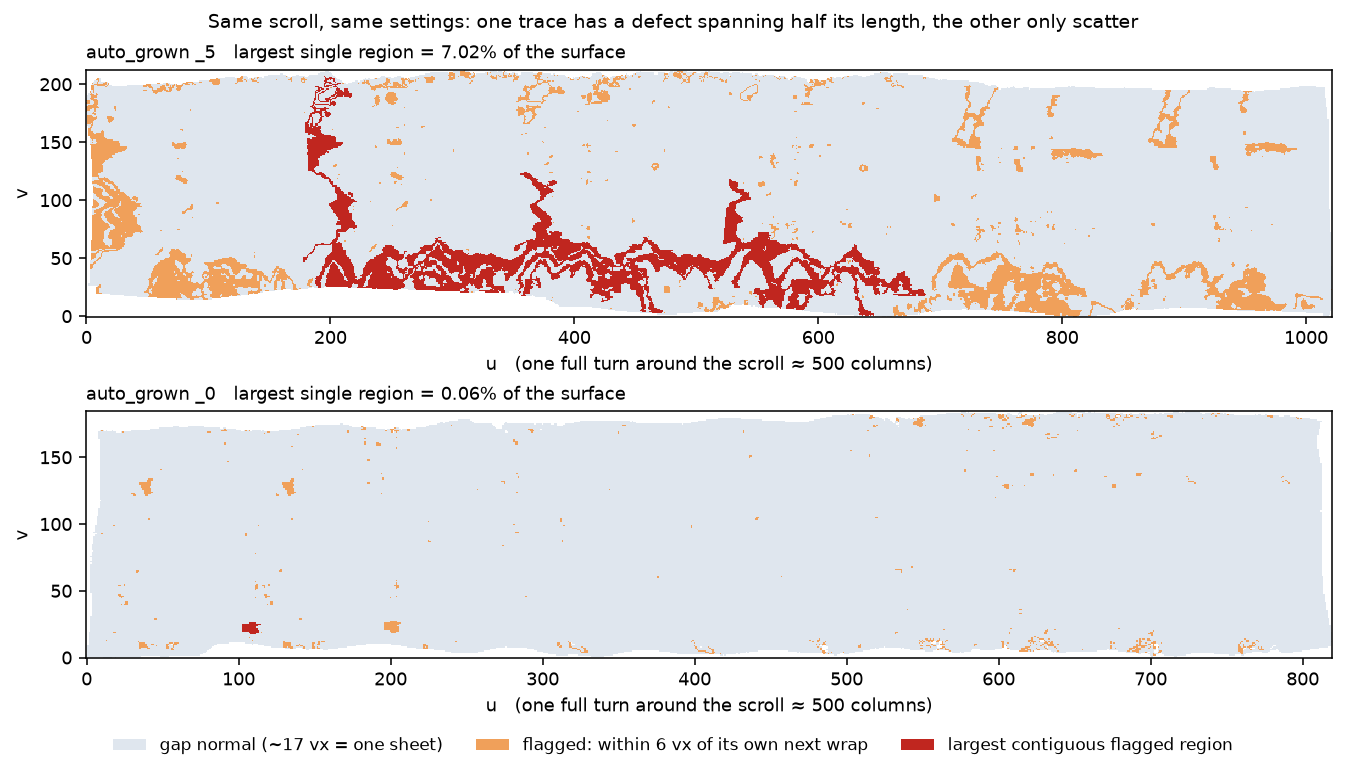
\includegraphics[width=\textwidth]{img/gap_maps.png}
\caption{Two traces from the same scroll under identical settings. The upper
has a single contiguous flagged region covering 7.02\% of its surface and
spanning roughly half its length; the lower has only scatter.}
\end{figure}

Across 19 analysed traces on two scrolls, two facts separate cleanly.

\textbf{Scattered flagging is normal.} The overall violation rate overlaps
between scrolls (\texttt{PHerc0172} 0.36--6.60\%, \texttt{PHerc0814}
0.32--6.77\%). Taken alone it distinguishes nothing, and should not be read as a
defect signature.

\textbf{Concentration does not.} Measured as the largest contiguous flagged
region as a fraction of analysed surface, one trace stands at 7.02\% against
1.52\% for the next and 0.06\% for the lowest. That ordering is the usable
output: it says which trace a human should open first.

\begin{figure}[h]
\centering
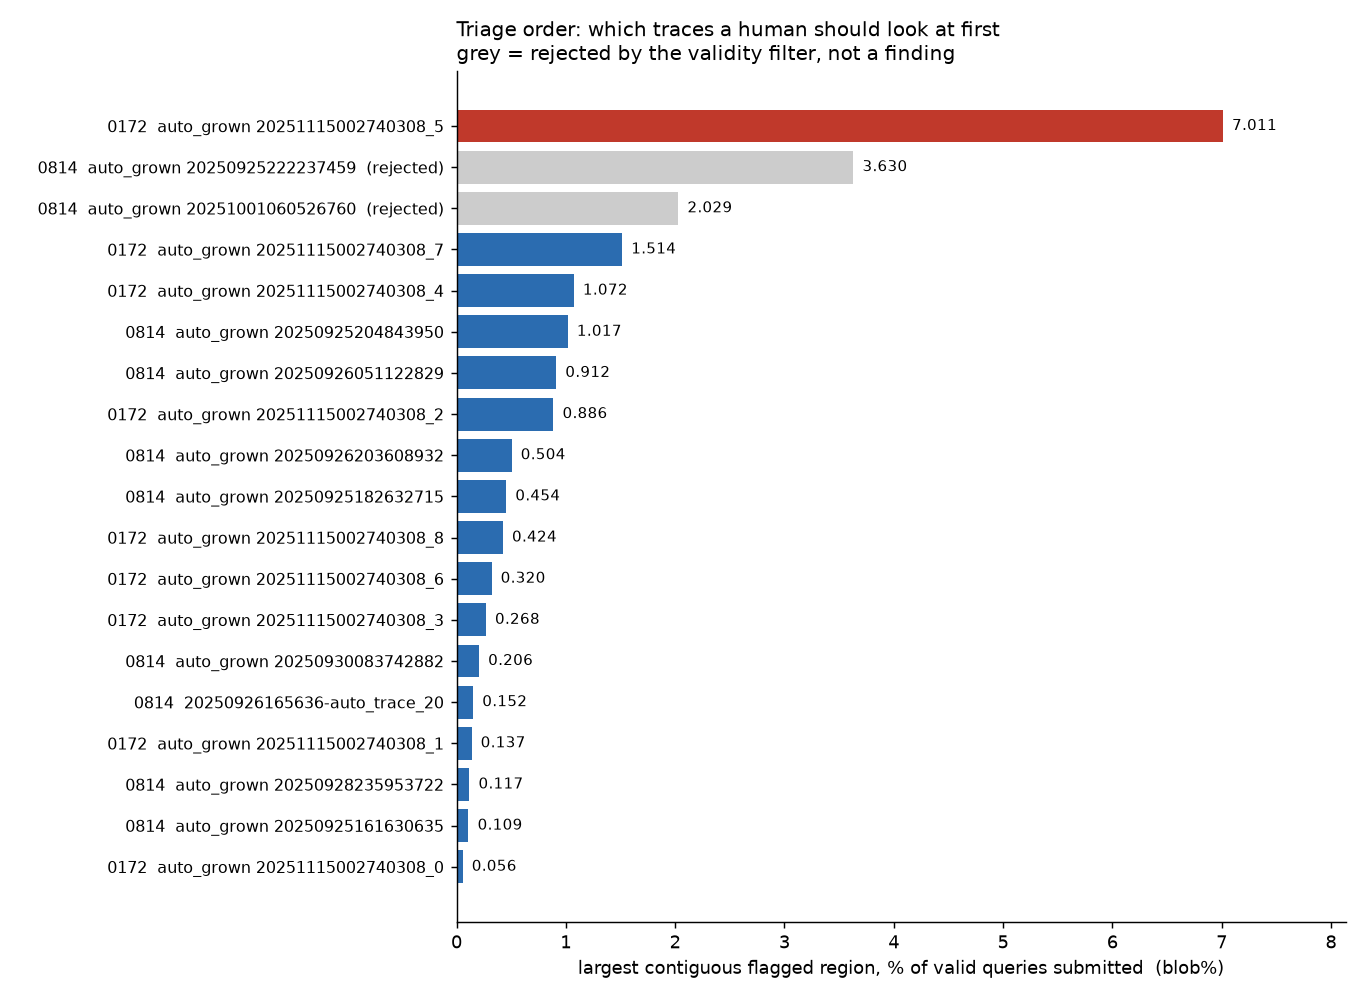
\includegraphics[width=0.85\textwidth]{img/triage_ranking.png}
\caption{All 19 analysed traces ordered by concentration. Rows rejected by the
validity filter are greyed rather than removed.}
\end{figure}

\section{What this does not establish}

Stated plainly, because stronger versions of each claim were tested and dropped.

\textbf{These regions are not proven to be errors.} Three independent attempts
to confirm them against the CT volume failed. The strongest, a missed-sheet test
asking whether a nearby bright band is occupied by no part of the trace, gave
Cohen's $d = 0.245$ at $p = 0.0496$ --- in the predicted direction, but far too
small to certify any individual region. The geometry is solid; the
interpretation as a defect is not established.

\textbf{No claim is made that the published output violates the criterion of
the grower that produced it.} \texttt{volume-cartographer} defines
\texttt{same\_surface\_th = 2.0} and rejects growth candidates within that
distance of already-traced surface, which is why 2.0 voxels is reported as a
column. But the published Scroll~5 meshes pass through private artifacts,
flattening and reconstruction before release, so their provenance to any
specific revision is not established. What can be said is narrower and still
useful: no stage re-checks that criterion after optimisation.

\textbf{The sample is small.} The nine Scroll~5 \texttt{auto\_grown} traces are
partitions of a single artifact, not nine independent runs. The effective sample
is one run plus eight \texttt{PHerc0814} segments. Two scrolls is not enough to
characterise a pipeline.

\textbf{Known limitations.} The exclusion width is fixed rather than adapted to
each trace's turn period; exclusion is by grid column rather than mesh geodesic
distance; and single-wrap patches cannot be analysed at all.

\section{Reproducing}

Everything below runs from published data with no credentials.

{\small
\begin{verbatim}
    uv sync
    clang++ -O3 -std=c++17 -pthread \
        -o engines/atlas_query engines/atlas_query.cpp
    uv run pytest -q

    uv run python -m windcheck.fetch --sample PHerc0172
    uv run windcheck calibrate data/scroll5_tifxyz
    uv run windcheck selfgap   data/scroll5_tifxyz --json report.json
\end{verbatim}
}

\texttt{data/MANIFEST.json} pins every input file by S3 key, byte count and
SHA-256, so a result can be traced to exact bytes. The outputs quoted in this
document are committed under \texttt{sample\_outputs/}, each headed by the
command that produced it.

Five tests run without any data. Each is tied to a mistake made during
development: the accelerated search against brute force; certification of the
search radius; true surface separation against grid pitch; the null control; and
missing-cell handling.

\section*{Availability}

Source, figures and sample outputs: \texttt{https://github.com/joe-carr-data/windcheck}\\
Licence: MIT.

\end{document}
